\documentclass{article}
\usepackage{iclr2026_conference,times}

\input{math_commands.tex}

\usepackage{booktabs}
\usepackage{graphicx}
\usepackage{hyperref}
\usepackage{url}

\title{Source-Private Tool-Trace Packets for Rate-Capped Evidence Communication}

\author{Anonymous Authors}

\newcommand{\diag}{\texttt{REPAIR\_DIAG}}
\newcommand{\tracehint}{\texttt{trace\_no\_hint}}

\begin{document}

\maketitle

\begin{abstract}
Agent systems can benefit when one model uses private evidence observed by
another without relaying a full trace. We formalize this as source-private
evidence communication with decoder side information: a target agent receives
the public task and a candidate pool, while a source agent observes private
execution evidence and sends a rate-capped message. We instantiate this setting
with a hidden-repair benchmark where the target selects among public repair
candidates and the source observes private tool-trace diagnostics. A compact
explicit \diag{} packet improves target-side candidate selection from 25\% to
80.8--100.0\% across four frozen 500-example core and held-out-family
surfaces. Zero-source, shuffled-source, random same-byte, answer-only,
answer-masked, target-derived, same-byte structured relay, helper/no-log, and
trace-removed controls remain at target-only. Model-produced packets average
1.55--2.00 bytes, compared with roughly 366--374 bytes and 34 tokens for full
hidden-log relay. A small Qwen3 target-decoder smoke further shows that the
packet can be consumed by a model-mediated target selector, not only by a
hand-coded lookup. The result is a narrow but reproducible positive method:
explicit source-private tool-trace packets can transmit the benchmark's hidden
diagnostic evidence under the controls tested here and with explicit rate
accounting.
\end{abstract}

\section{Introduction}

Multi-agent and cross-model systems increasingly divide work across components
with asymmetric information. A tool-using source agent may observe execution
traces, retrieval results, private memory, or environment feedback unavailable
to the target agent that must make the final decision. Full trace relay is a
simple interface, but it can be wasteful when the target already has useful side
information such as a candidate pool or cached prior.

We study a narrower question: can a source agent send a compact, auditable
message that changes the target's decision only when matched private source
evidence is present? This framing follows distributed source coding and
rate-distortion intuitions: a sender can communicate fewer bits when the decoder
has side information, and the objective is task distortion at a communication
rate rather than reconstruction of the whole source state
\citep{slepian1973noiseless,wyner1976rate,shannon1959coding}. Here, the
target's candidate pool is decoder side information, and the source packet is
evaluated by downstream selector accuracy under source controls.

We instantiate this idea in hidden-repair candidate selection. The target
receives a public repair issue, buggy implementation, and four public repair
candidates. The source receives a private hidden-test/tool trace containing an
explicit repair diagnostic. The source model emits a compact \diag{} packet,
and the target-side decoder uses the packet and public candidate metadata to
select a repair candidate. The packet is interpretable and byte-counted.

The contribution is intentionally scoped. We do not claim unstructured latent
transfer, raw-log repair reasoning, or universal cross-model communication. We
claim that a rate-capped source-private packet can carry the benchmark's hidden
diagnostic evidence to a target-side candidate decoder under the controls
tested here.

\section{Problem Setup}

Each example has public task and candidate information $X$, target-side state
$T$, source-private evidence $S$, a rate-capped source message $M$, and a
decoder $D(X,T,M)$ that selects a final candidate. The target never sees $S$
directly except in full-relay oracle baselines. A method is counted as
communication only if $D(X,T,M_{\mathrm{matched}})$ improves over no-source and
source-destroying controls:
zero-source, shuffled-source, random same-byte, answer-only, answer-masked,
target-derived, and same-byte relay messages.

We report selector accuracy, candidate-pool recall, exact ID parity, packet
validity, paired uncertainty, bytes/tokens, and source-control deltas.

\begin{figure}[t]
  \centering
  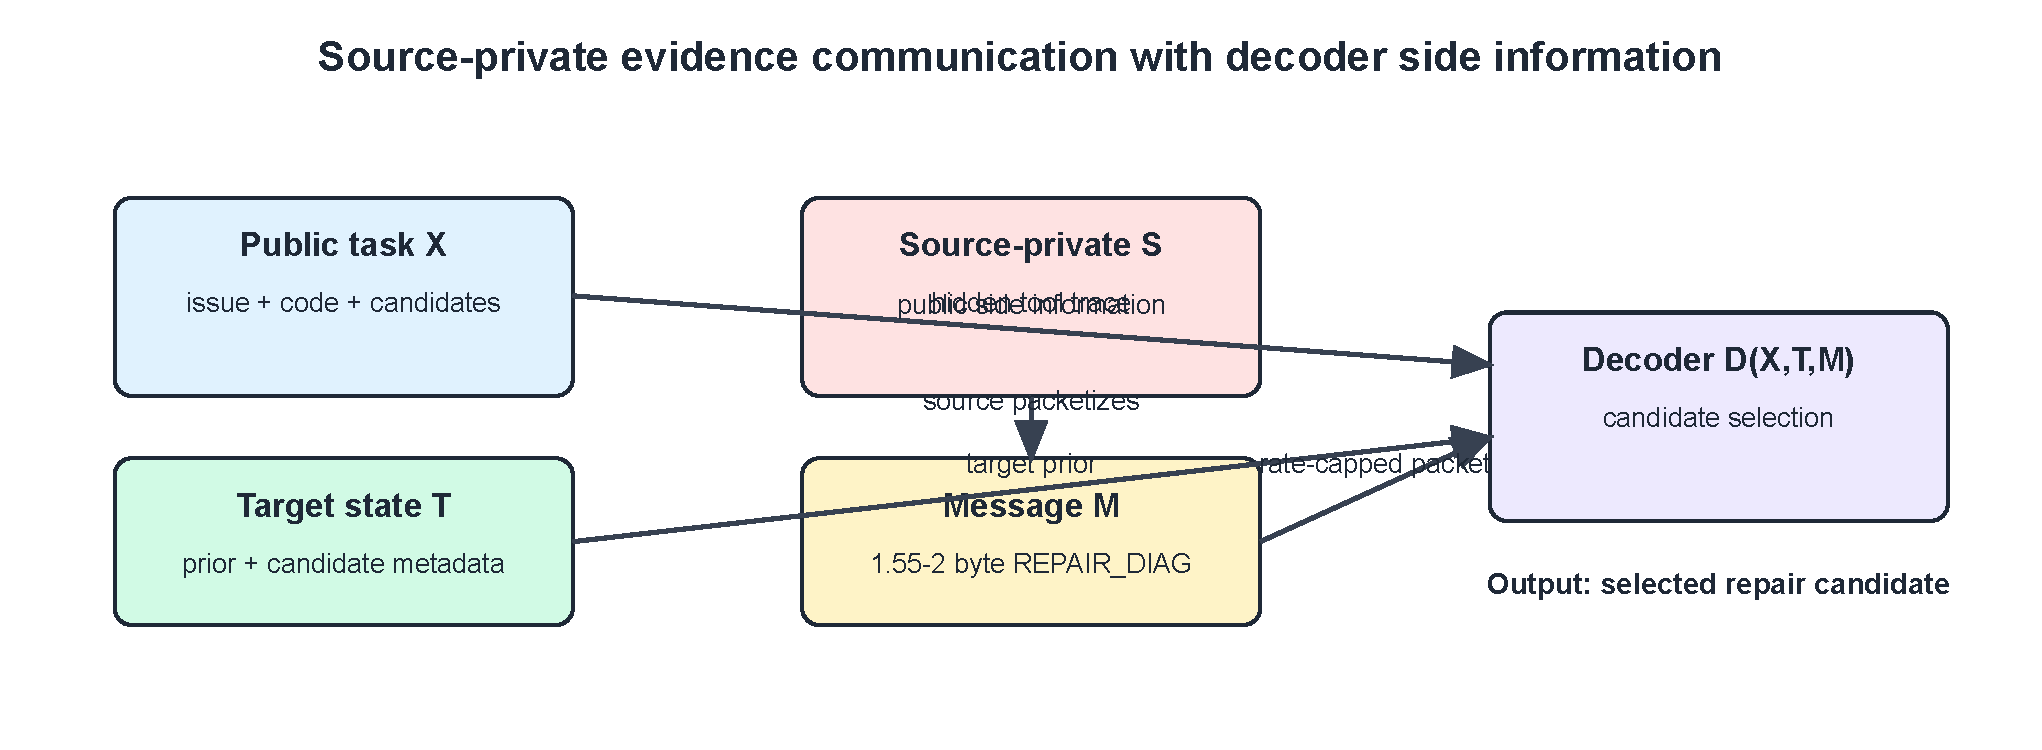
\includegraphics[width=\linewidth]{../../results/source_private_tool_trace_latex_or_figures_20260430/source_private_setup.pdf}
  \caption{Source-private evidence communication with decoder side information.
  The source observes private evidence $S$ and sends a rate-capped packet $M$.
  The target combines public state $X$, candidate state $T$, and $M$ to select a
  candidate.}
  \label{fig:setup}
\end{figure}

\section{Benchmark}

The hidden-repair benchmark contains deterministic Python repair tasks. Each
example has public issue text, a buggy implementation, four public candidate
repairs, one gold candidate in the pool, and a source-private hidden-test/tool
log. Public candidate metadata includes \texttt{handles\_repair\_diag=<code>}.
The private source log contains \texttt{private\_tool\_trace: REPAIR\_DIAG=<code>}.

The target prior solves exactly one quarter of examples. The main surfaces are
a strict-small 160-example slice, a 500-example core slice, a 500-example
held-out repair-family slice, and seed repeats over core seeds 29/31 and
held-out seeds 30/32. Deterministic surfaces have candidate-pool recall 1.0, so
reported improvements are selector improvements.

\section{Method}

The source model receives a private hidden-test log and emits only a compact
repair packet. In the main model-mediated condition, \tracehint{}, the private
diagnostic line remains in the private log, but the copied helper line and hint
are removed. Invalid packets fall back to the target prior.

The target-side protocol decoder receives the public candidate pool and packet.
If the packet is a valid diagnostic matching exactly one candidate's
\texttt{handles\_repair\_diag} metadata, the decoder selects that candidate;
otherwise it returns the target-prior candidate. This design makes the
communication channel auditable, but it is protocol-shaped rather than a
learned latent bridge. We therefore include a Qwen3 target-decoder smoke
ablation in Section~\ref{sec:target-decoder}.

\section{Baselines and Controls}

We compare against target-only and target-wrapper/no-source baselines; zero,
shuffled, random same-byte, and target-derived source-destroying controls;
answer-only and answer-masked leakage controls; matched-byte hidden-log prefix,
JSON, and free-text relays; full hidden-log and full diagnostic oracles; and
trace-component ablations including diagnostic-masked, expected/actual-masked,
test-name-masked, and trace-removed logs.

\section{Results}

Table~\ref{tab:main} reports model-produced source packets across four frozen
500-example surfaces. Qwen3 reaches 80.8--92.4\% accuracy and Phi-3 reaches
100\%, while target-only remains 25\% and source-destroying controls remain
near target-only.

\begin{table}[t]
\centering
\small
\begin{tabular}{llrrrrrr}
\toprule
Surface & Source model & Matched & Target & Control & Valid & Bytes & 95\% CI \\
\midrule
core 29 & Qwen3-0.6B & 404/500 & 125/500 & 126/500 & 0.776 & 1.55 & [0.516,0.600] \\
core 29 & Phi-3-mini & 500/500 & 125/500 & 126/500 & 1.000 & 2.00 & [0.714,0.788] \\
core 31 & Qwen3-0.6B & 404/500 & 125/500 & 128/500 & 0.776 & 1.55 & [0.516,0.602] \\
core 31 & Phi-3-mini & 500/500 & 125/500 & 128/500 & 1.000 & 2.00 & [0.710,0.786] \\
held-out 30 & Qwen3-0.6B & 461/500 & 125/500 & 129/500 & 0.864 & 1.73 & [0.632,0.712] \\
held-out 30 & Phi-3-mini & 500/500 & 125/500 & 129/500 & 1.000 & 2.00 & [0.710,0.788] \\
held-out 32 & Qwen3-0.6B & 462/500 & 125/500 & 126/500 & 0.860 & 1.72 & [0.634,0.716] \\
held-out 32 & Phi-3-mini & 500/500 & 125/500 & 126/500 & 1.000 & 2.00 & [0.710,0.786] \\
\bottomrule
\end{tabular}
\caption{Model-mediated source-packet rows over four frozen 500-example
surfaces. Control is the best source-destroying control on that surface.
Intervals are paired bootstrap 95\% intervals for matched minus target.}
\label{tab:main}
\end{table}

Removing the private trace diagnostic kills the effect: Qwen3
\texttt{raw\_log\_no\_trace} returns to 25\% with zero valid packets on all
four surfaces.

\section{Threat Model Results}

At the 2-byte packet budget, deterministic reviewer-risk controls remain at
target-only while full-log and diagnostic oracles reach 100\%. Table~\ref{tab:controls}
summarizes representative core and held-out surfaces.

\begin{table}[t]
\centering
\small
\begin{tabular}{lrrrrrrrr}
\toprule
Surface & Matched & Target & Zero & Shuffled & Random & JSON & Free text & Diag-masked \\
\midrule
core 29 & 1.000 & 0.250 & 0.250 & 0.250 & 0.254 & 0.250 & 0.250 & 0.250 \\
held-out 30 & 1.000 & 0.250 & 0.250 & 0.250 & 0.254 & 0.250 & 0.250 & 0.250 \\
\bottomrule
\end{tabular}
\caption{Deterministic threat-model rows at the 2-byte packet budget. Same-byte
JSON/free-text relays and diagnostic-masked logs stay at target-only.}
\label{tab:controls}
\end{table}

\section{Rate and Systems Analysis}

The method's systems value is rate efficiency. Model-produced packets average
1.55--2.00 bytes and roughly one token. Full hidden-log relay reaches oracle
accuracy but costs roughly 366--374 bytes and 34 tokens per example. Structured
JSON and free-text relays fail at 2 bytes but become oracles at 32 bytes because
the diagnostic is then visible in parseable form.

\begin{figure}[t]
  \centering
  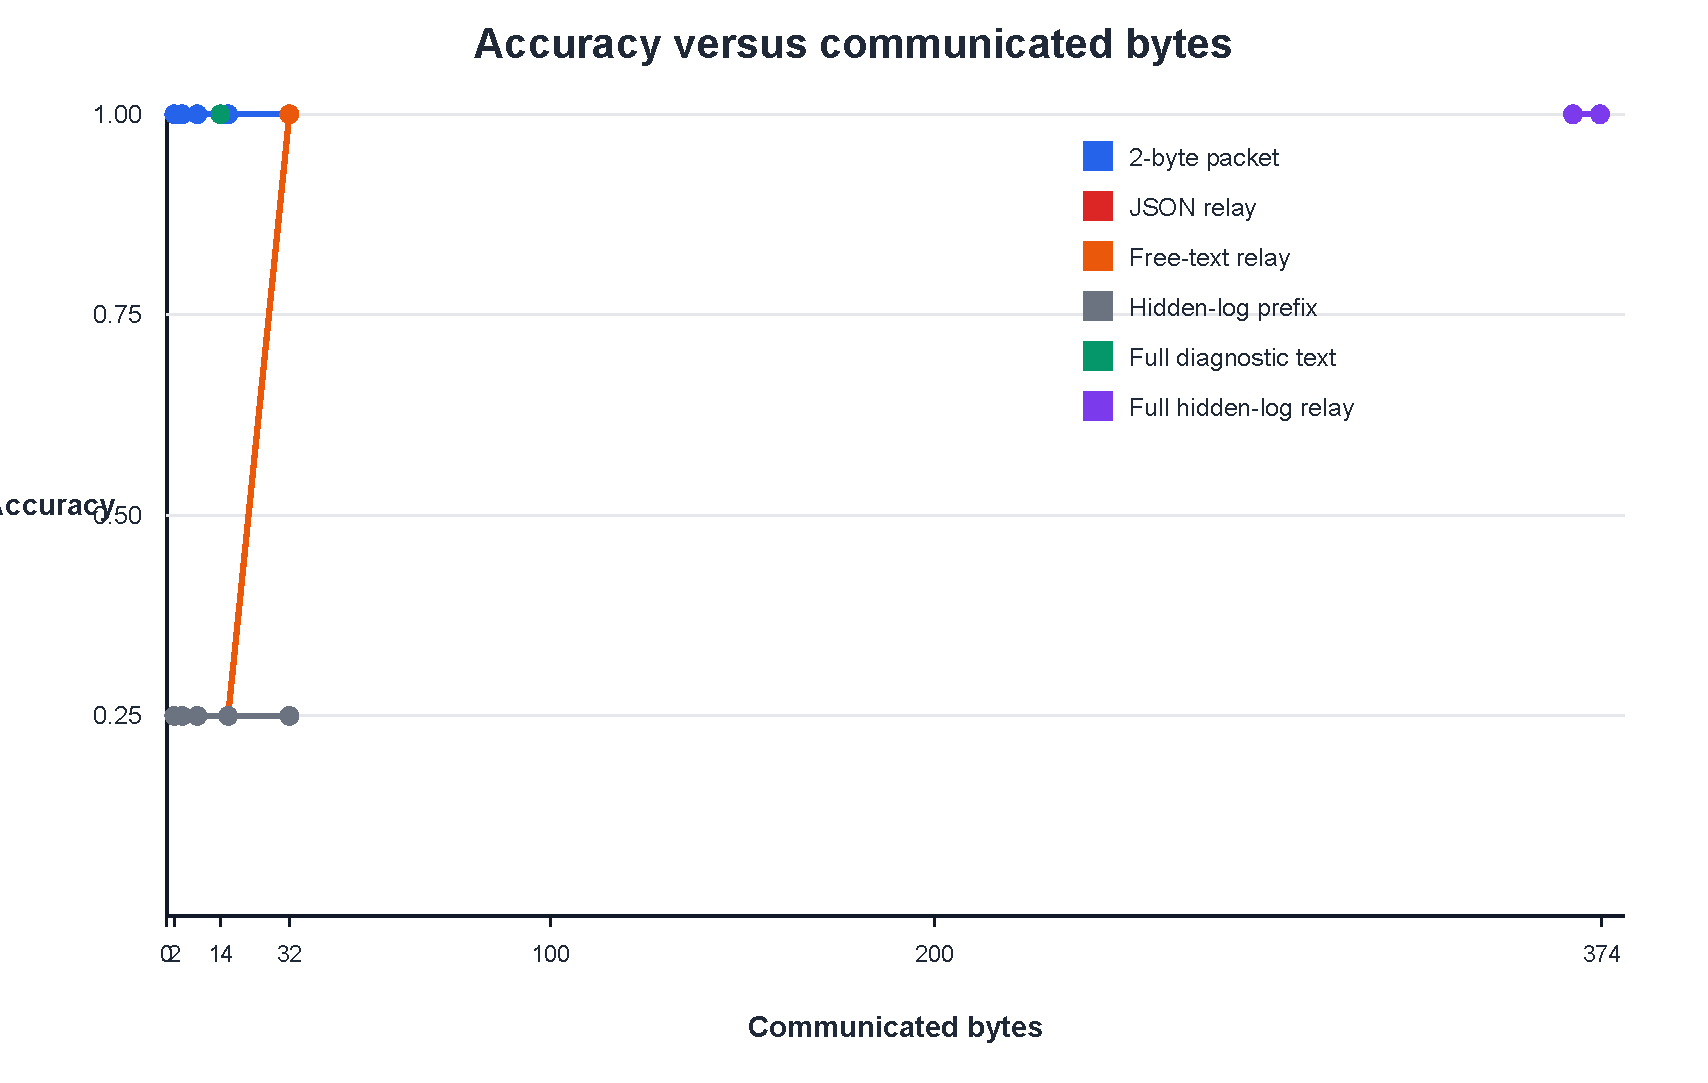
\includegraphics[width=0.9\linewidth]{../../results/source_private_tool_trace_latex_or_figures_20260430/rate_curve.pdf}
  \caption{Accuracy versus communicated bytes, averaged over representative
  core and held-out reviewer-risk surfaces. Structured text relay becomes an
  oracle when granted enough bytes, while compact packets occupy the
  far-left-rate regime.}
  \label{fig:rate}
\end{figure}

\section{Target-Decoder Smoke}
\label{sec:target-decoder}

To test whether the hard-coded target lookup is essential, we replace it with
Qwen3-0.6B acting as a target-side selector. The model receives the target-prior
fallback label, source packet, candidate labels, and candidate diagnostic
metadata. On a 16-example core slice, matched packets reach 0.688 versus 0.250
target/control. On a 32-example held-out slice, matched packets reach 0.750
versus 0.250 target and 0.281 best control. This is a smoke ablation, not the
main evidence, but it reduces the hand-coded lookup concern.

\section{Interpretability}

The packet channel is directly auditable in this benchmark. The packet is a
two-character diagnostic code; target candidate metadata states which diagnostic
each candidate handles; and component-masking controls identify the private
trace field that carries the signal. Failures can be audited as invalid source
packets, fallback-to-prior cases, or target-decoder selection mistakes.

\section{Related Work}

Distributed source coding motivates our setup: Slepian-Wolf and Wyner-Ziv
coding show that a sender can communicate fewer bits when the decoder has side
information \citep{slepian1973noiseless,wyner1976rate}; rate-distortion theory
frames evaluation as distortion at a communication rate
\citep{shannon1959coding}. Semantic communication motivates task-oriented
utility per transmitted bit \citep{xie2021deep}. Tool-using agents such as
ReAct and Toolformer motivate private tool traces as source evidence
\citep{yao2022react,schick2023toolformer}. VLM connectors and JEPA-style
objectives motivate future learned bottlenecks and anti-collapse diagnostics
\citep{alayrac2022flamingo,li2023blip2,assran2023ijepa,bardes2021vicreg}.
Cache and activation transfer methods such as C2C and KV communication are
related competitors for internal-state communication, while our method focuses
on explicit source-private evidence packets.

\section{Limitations}

The main limitation is scope. Candidate metadata exposes the diagnostic mapping,
and the primary decoder is deterministic and protocol-shaped. The target-decoder
smoke reduces this concern but remains small. The benchmark is synthetic;
held-out families and seed repeats reduce template-specific concerns but do not
replace real tool or retrieval workflows. Structured text relay becomes an
oracle when granted enough bytes. Finally, this work does not show unstructured
latent transfer or universal cross-model communication.

\section{Conclusion}

We present a scoped positive method for source-private evidence communication.
A source model reads private tool-trace diagnostics and emits a compact explicit
packet. A target-side candidate decoder combines that packet with public
candidate metadata to select the correct repair. The method is reproducible,
interpretable, rate-accounted, and stable across the tested frozen 500-example
surfaces, held-out repair families, seed repeats, source-destroying controls,
structured relay baselines, and a small target-LLM decoder ablation.

\bibliography{source_private_tool_trace}
\bibliographystyle{iclr2026_conference}

\appendix

\section{Claim Boundary}

We claim that explicit source-private tool-trace packets can communicate hidden
diagnostic evidence to a target-side candidate decoder under rate constraints.
We do not claim raw-log repair inference, learned latent transfer, universal
cross-model communication, or unconstrained repair generation.

\section{Artifacts}

Main result artifacts are tracked in the source-private tool-trace results
folders. The reproduction entry points are the hidden-repair packet
generator/evaluator, model packet extractor, baseline-pack builder, figure
builder, and target-decoder smoke scripts; exact commands and paths are recorded
in the artifact manifests.

\end{document}
